\documentclass[xcolor=dvipsnames,handout]{beamer}
\usetheme{Owlie}

\def\CC{{C\nolinebreak[4]\hspace{-.05em}\raisebox{.2ex}{++}}}
\title[\CC]{Programmare in \CC}
\author[A.~Saltini]{Alessandro Saltini}
\institute[LS Tassoni]{Liceo Scientifico Statale ``A.~Tassoni''}
\date{A.S.~2015/2016}
\setlength{\parindent}{0pt}

\input{headers/default}
\usepackage[
  list-units=single,
  range-units=single,
  multi-part-units=single,
  exponent-product=\cdot,
  per-mode=fraction,
  math-ohm=\mathrm{\Omega},
  text-ohm={\ensuremath{\mathrm{\Omega}}},
  retain-explicit-plus=true,
  retain-zero-exponent,
  binary-units=true
]{siunitx}
\AtBeginDocument{\sisetup{math-rm=\mathrm, text-rm=\rmfamily}}
\DeclareSIUnit{\atp}{at.\percent}
\DeclareSIUnit{\magn}{\ensuremath{\times}}
\DeclareSIUnit{\rpm}{rpm}
\DeclareSIUnit{\nit}{nt}
\DeclareSIUnit{\talbot}{Tb}

% \input{headers/bibliography}
\usepackage{tikz}
\usetikzlibrary{
  positioning,
  shapes,
  shapes.geometric,
  shapes.symbols,
  shapes.misc,
  shadows,
  arrows,
  fit,
  decorations,
  patterns,
  mindmap,
  calc
}

\usepackage{readarray}
\usepackage{ifthen}
\usepackage{pgfplots}
\pgfplotsset{compat=newest}
\usepackage{chemfig}

\tikzset{
    begin/.style={
        draw,
        rectangle,
        rounded corners,
        very thick,
        draw=MidnightBlue!80!black,
        fill=MidnightBlue!50
    },
    input/.style={ % requires library shapes.geometric
        draw,
        trapezium,
        trapezium left angle=60,
        trapezium right angle=120,
        very thick,
        draw=BrickRed!80!black,
        fill=BrickRed!50
    },
    output/.style={ % requires library shapes.geometric
        draw,
        trapezium,
        trapezium left angle=60,
        trapezium right angle=120,
        very thick,
        draw=Fuchsia!80!black,
        fill=Fuchsia!50
    },
    operation/.style={
        draw,
        rectangle,
        very thick,
        draw=BurntOrange,
        fill=BurntOrange!50
    },
    loop/.style={ % requires library shapes.misc
        draw,
        chamfered rectangle,
        chamfered rectangle xsep=2cm,
        very thick,
        draw=ForestGreen!80!black,
        fill=ForestGreen!50
    },
    decision/.style={ % requires library shapes.geometric
        draw,
        diamond,
        aspect=#1,
        very thick,
        draw=ForestGreen!80!black,
        fill=ForestGreen!50
    },
    decision/.default=2,
    print/.style={ % requires library shapes.symbols
        draw,
        tape,
        tape bend top=none
    },
    connection/.style={
        draw,
        thick,
        circle,
        fill=MidnightBlue
    },
    process rectangle outer width/.initial=0.15cm,
    predefined process/.style={
        rectangle,
        draw,
        append after command={
        \pgfextra{
          \draw
          ($(\tikzlastnode.north west)-(0,0.5\pgflinewidth)$)--
          ($(\tikzlastnode.north west)-(\pgfkeysvalueof{/tikz/process rectangle outer width},0.5\pgflinewidth)$)--
          ($(\tikzlastnode.south west)+(-\pgfkeysvalueof{/tikz/process rectangle outer width},+0.5\pgflinewidth)$)--
          ($(\tikzlastnode.south west)+(0,0.5\pgflinewidth)$);
          \draw
          ($(\tikzlastnode.north east)-(0,0.5\pgflinewidth)$)--
          ($(\tikzlastnode.north east)+(\pgfkeysvalueof{/tikz/process rectangle outer width},-0.5\pgflinewidth)$)--
          ($(\tikzlastnode.south east)+(\pgfkeysvalueof{/tikz/process rectangle outer width},0.5\pgflinewidth)$)--
          ($(\tikzlastnode.south east)+(0,0.5\pgflinewidth)$);
        }
        },
        text width=#1,
        align=center
    },
    predefined process/.default=1.75cm,
    man op/.style={ % requires library shapes.geometric
        draw,
        trapezium,
        shape border rotate=180,
        text width=2cm,
        align=center,
    },
    extract/.style={
        draw,
        isosceles triangle,
        isosceles triangle apex angle=60,
        shape border rotate=90
    },
    merge/.style={
        draw,
        isosceles triangle,
        isosceles triangle apex angle=60,
        shape border rotate=-90
    },
    arrow/.style={
        thick,
        ->,
        >=stealth
    },
}


\usepackage{listings}

\lstset{ %
  backgroundcolor=\color{White},          % choose the background color; you must add \usepackage{color} or \usepackage{xcolor}
  basicstyle=\footnotesize\ttfamily,      % the size of the fonts that are used for the code
  breaklines=true,                        % sets automatic line breaking
  commentstyle=\color{OliveGreen},        % comment style
  frame=L,                                % adds a frame around the code
  keepspaces=true,                        % keeps spaces in text, useful for keeping indentation of code (possibly needs columns=flexible)
  %keywordstyle=\color{blue},             % keyword style
  language=C++,                           % the language of the code
  numbers=left,                           % where to put the line-numbers; possible values are (none, left, right)
  numbersep=10pt,                         % how far the line-numbers are from the code
  numberstyle=\tiny\color{Gray},          % the style that is used for the line-numbers
  rulecolor=\color{Black},                % if not set, the frame-color may be changed on line-breaks within not-black text (e.g. comments (green here))
  stepnumber=1,                           % the step between two line-numbers. If it's 1, each line will be numbered
  stringstyle=\color{BurntOrange},        % string literal style
  tabsize=2,                              % sets default tabsize to 2 spaces
  showstringspaces=false,                 % underline spaces within strings only
}

% \input{headers/fancy}

\begin{document}

\begin{frame}[noframenumbering]
  \titlepage
\end{frame}

\begin{frame}{L'informatica}
  \vfill
  \begin{itemize}
    \item L'informatica \alert{non} è
    \begin{itemize}
      \item saper usare un computer
      \item saper costruire/riparare un computer
      \item usare programmi scritti da altri
    \end{itemize}
    \vfill
    \item L'informatica è
    \begin{itemize}
      \item una branca della matematica
      \item lo studio dell'\alert{informazione}
      \item lo studio degli \alert{algoritmi}
      \item lo studio dei \alert{linguaggi di programmazione}
    \end{itemize}
  \end{itemize}
  \vfill
\end{frame}

\begin{frame}{L'informazione}
  \vfill
  \begin{itemize}
    \item L'informazione si misura in \alert{bit} (\alert{bi}nary digi\alert{t})
    \vfill
    \item \SI{1}{\bit} è la quantità di informazione necessaria a determinare una
    quantità che può essere \alert{0} o \alert{1}
    \vfill
    \item Il \alert{byte} è un multiplo del bit: \SI{1}{\byte} = \SI{8}{\bit}
    \vfill
    \item Due scale di multipli del byte:
    \begin{itemize}
      \item decimale: \si{\kilo\byte} (\(10^3\)), \si{\mega\byte} (\(10^6\)), \si{\giga\byte} (\(10^9\)), \si{\tera\byte} (\(10^{12}\)), \dots
      \item \alert{binaria}: \si{\kibi\byte} (\(2^{10}\)), \si{\mebi\byte} (\(2^{20}\)), \si{\gibi\byte} (\(2^{30}\)), \si{\tebi\byte} (\(2^{40}\)), \dots
    \end{itemize}
  \end{itemize}
  \vfill
\end{frame}

\begin{frame}{Algebra Booleana}
  \vfill
  \begin{itemize}
    \item L'algebra Booleana è l'algebra dei bit
    \vfill
    \item È un \alert{modello} della logica classica: 1 = vero, 0 = falso
    \vfill
    \item Insieme di base \(\mathcal{B} = \{ \; 0, 1 \; \}\)
    \vfill
    \item Tre operazioni fondamentali:
    \begin{itemize}
      \item \alert{not} (non): \(\lnot : \mathcal{B} \to \mathcal{B}\)
      \item \alert{and} (et): \(\land : \mathcal{B}^2 \to \mathcal{B}\)
      \item \alert{or} (vel): \(\lor : \mathcal{B}^2 \to \mathcal{B}\)
    \end{itemize}
  \end{itemize}
  \vfill
\end{frame}

\begin{frame}{Algebra Booleana}
  \begin{itemize}
      \item \alert{not} (non): \(\lnot\)
      \begin{itemize}
        \item \(\lnot 1 = 0\)
        \item \(\lnot 0 = 1\)
      \end{itemize}
      \vfill
      \item \alert{and} (et): \(\land\)
      \begin{itemize}
        \item \(1 \land 1 = 1\)
        \item \(1 \land 0 = 0\)
        \item \(0 \land 1 = 0\)
        \item \(0 \land 0 = 0\)
      \end{itemize}
      \vfill
      \item \alert{or} (vel): \(\lor\)
      \begin{itemize}
        \item \(1 \lor 1 = 1\)
        \item \(1 \lor 0 = 1\)
        \item \(0 \lor 1 = 1\)
        \item \(0 \lor 0 = 0\)
      \end{itemize}
  \end{itemize}
\end{frame}

\begin{frame}{Algebra Booleana}
  \vfill
  \begin{itemize}
    \item Combinando queste tre operazioni si possono ottenere tutte le altre
    operazioni possibili
    \vfill
    \item In realtà basta \alert{una} sola operazione, meno intuitiva:
    \begin{itemize}
      \item nand (\(\uparrow\))
      \item nor (\(\downarrow\))
    \end{itemize}
    \vfill
    \item Esistono circuiti \alert{elettrici} che realizzano materialmente queste
    operazioni logiche
    \begin{itemize}
      \item segnale ``alto'' = 1
      \item segnale ``basso'' = 0
    \end{itemize}
    \vfill
    \item Sono l'elemento di base dei computer
  \end{itemize}
  \vfill
\end{frame}

\begin{frame}{Rappresentazione decimale}
  \vfill
  \begin{itemize}
    \item Un numero in rappresentazione \alert{decimale} è espresso come combinazione
    di potenze di 10
    \[\num{1064} = \num{1e3} + \num{0e2} + \num{6e1} + \num{4e0}\]
    \item I coefficienti sono compresi tra 0 e 9 (\alert{minori} di 10)
    \vfill
    \item Il massimo numero con \(n\) cifre decimali è \(10^n - 1\)
    \vfill
    \item I numeri esistono indipendentemente dalla loro rappresentazione, è solo
    un modo di scriverli
  \end{itemize}
  \vfill
\end{frame}

\begin{frame}{Rappresentazione binaria}
  \vfill
  \begin{itemize}
    \item La rappresentazione \alert{binaria} utilizza le potenze di 2
    \[\num[group-digits = false]{10110} = \num[exponent-base = 2]{1e4} + \num[exponent-base = 2]{0e3}
    + \num[exponent-base = 2]{1e2} + \num[exponent-base = 2]{1e1} + \num[exponent-base = 2]{0e0}\]
    \item I coefficienti sono soltanto 0 e 1 (\alert{minori} di 2)
    \vfill
    \item Il massimo numero con \(n\) cifre binarie è \(2^n - 1\)
    \vfill
    \item Ogni cifra è rappresentabile da un \alert{bit}
    \begin{itemize}
      \item \(n\) cifre \(\Rightarrow\) \(n\) bit
    \end{itemize}
  \end{itemize}
  \vfill
\end{frame}

\begin{frame}{Rappresentazione binaria}
  \vfill
  \begin{itemize}
    \item I computer memorizzano i numeri in binario
    \vfill
    \item Le operazioni tra essi vengono svolte da appositi circuiti, basati
    sulle operazioni Booleane
    \vfill
    \item Ogni operazione richiede un certo tempo
    \vfill
    \item Limiti di memoria/tempo impediscono di operare con numeri arbitrariamente
    grandi
  \end{itemize}
  \vfill
\end{frame}

\begin{frame}{Rappresentazione binaria}
  \vfill
  \begin{itemize}
    \item I numeri negativi devono memorizzare anche il segno
    \vfill
    \item Costo di \SI{1}{\bit} aggiuntivo
    \begin{itemize}
      \item \(s = 0 \Rightarrow +\)
      \item \(s = 1 \Rightarrow -\)
    \end{itemize}
    \vfill
    \item Spesso si ricorre a rappresentazioni alternative
    \begin{itemize}
      \item rimozione di ambiguità tra \(+0\) e \(-0\)
      \item facilità di calcolo
      \item occupano comunque \SI{1}{\bit} in più
    \end{itemize}
  \end{itemize}
  \vfill
\end{frame}

\begin{frame}{Rappresentazione binaria}
  \vfill
  \begin{itemize}
    \item La parte frazionaria è problematica da rappresentare
    \[\num[group-digits = false]{1.1011} = \num[exponent-base = 2]{1e0} + \num[exponent-base = 2]{1e-1}
    + \num[exponent-base = 2]{0e-2} + \num[exponent-base = 2]{1e-3} + \num[exponent-base = 2]{1e-4}\]
    \item Non tutti i numeri con rappresentazione decimale finità hanno rappresentazione
    binaria finita
    \vfill
    \item Non possiamo memorizzare infinite cifre
    \begin{itemize}
      \item Impossibile rappresentare i numeri irrazionali
      \item Non tutti i numeri razionali sono rappresentabili
    \end{itemize}
  \end{itemize}
  \vfill
\end{frame}

\begin{frame}{Rappresentazione binaria}
  \vfill
  \begin{itemize}
    \item Richiamiamo la notazione scientifica
    \[\num{1064.15} = \num{1.06415e3}\]
    \item Generalizzabile in binario come
    \[\num[group-digits = false]{110.1011} = \num[exponent-base = 2,group-digits = false]{1.101011e2}\]
    \item La \alert{prima} cifra della rappresentazione scientifica binaria è \alert{sempre 1}, non serve memorizzarla
  \end{itemize}
  \vfill
\end{frame}

\begin{frame}{Rappresentazione binaria}
  \vfill
    \[\num[group-digits = false]{110.1011} = \num[exponent-base = 2,group-digits = false]{1.101011e2}\]
  \begin{itemize}
    \item La parte dopo la virgola è detta \alert{mantissa} o \alert{significando}, è un numero intero
    \vfill
    \item L'\alert{esponente} di 2 è un numero intero
    \vfill
    \item Un numero frazionario viene rappresentato come coppia di numeri interi
    \begin{itemize}
      \item bit del significando \(\Rightarrow\) precisione
      \item bit dell'esponente \(\Rightarrow\) range
    \end{itemize}
  \end{itemize}
  \vfill
\end{frame}

\begin{frame}{Architettura di von Neumann}
  \vfill
  \begin{center}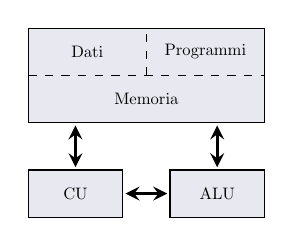
\begin{tikzpicture}[scale=0.6, every node/.style={scale=0.6}]
    \filldraw[fill=MidnightBlue!10!white] (0,0) rectangle ++(5,2);
    \draw[dashed] (0,1) -- (5,1) (2.5,1) -- (2.5,2);
    \filldraw[fill=MidnightBlue!10!white] (0,-2) rectangle ++(2,1);
    \filldraw[fill=MidnightBlue!10!white] (3,-2) rectangle ++(2,1);
    \path (2.5,0.5) node {Memoria}
          (1.25,1.5) node {Dati}
          (3.75,1.5) node {Programmi}
          (1,-1.5) node {CU}
          (4,-1.5) node {ALU};
    \draw[stealth-stealth,very thick,shorten >=1pt,shorten <=1pt] (2,-1.5) -- (3,-1.5);
    \draw[stealth-stealth,very thick,shorten >=1pt,shorten <=1pt] (1,-1) -- (1,0);
    \draw[stealth-stealth,very thick,shorten >=1pt,shorten <=1pt] (4,-1) -- (4,0);
  \end{tikzpicture}\end{center}
  \vfill
  \begin{itemize}
    \item Memoria unica per dati e programmi
    \vfill
    \item CU (Control Unit): assegna e gestisce risorse
    \vfill
    \item ALU (Arithmetic Logic Unit): compie operazioni
    \vfill
    \item ALU + CU = CPU (Central Processing Unit)
  \end{itemize}
  \vfill
\end{frame}

\begin{frame}{CPU}
  \vfill
  \begin{itemize}
    \item La CPU esegue istruzioni \alert{semplici}
    \vfill
    \item Istruzione tipo:
    \begin{itemize}
      \item che operazione fare
      \item indirizzi di memoria degli operandi
      \item indirizzi di memoria dei risultati
    \end{itemize}
    \vfill
    \item Le istruzioni sono codificate come numeri binari
    \vfill
    \item Le istruzioni eseguibili dipendono dal tipo di CPU
  \end{itemize}
  \vfill
\end{frame}

\begin{frame}{Assembly}
  \vfill
  \begin{itemize}
    \item I linguaggi \alert{assembly} hanno una corrispondenza 1-ad-1
    con le istruzioni della macchina
    \vfill
    \item Le istruzioni vengono ``tradotte'' da numeri binari a parole comprensibili
    ad un essere umano
    \vfill
    \item Un programma in assembly è una lista di istruzioni che la CPU eseguirà
    nell'ordine in cui appaiono
    \vfill
    \item CPU diverse hanno linguaggi assembly diversi
  \end{itemize}
  \vfill
\end{frame}

\begin{frame}{Assembly}
  \vfill
  \begin{center}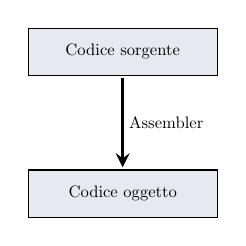
\begin{tikzpicture}[scale=0.6, every node/.style={scale=0.6}]
    \filldraw[fill=MidnightBlue!10!white] (0,0) rectangle ++(4,1);
    \filldraw[fill=MidnightBlue!10!white] (0,-3) rectangle ++(4,1);
    \path (2,0.5) node {Codice sorgente}
          (2,-2.5) node {Codice oggetto};
    \draw[-stealth,very thick,shorten >=1pt,shorten <=1pt] (2,0) -- node[right] {Assembler} (2,-2);
  \end{tikzpicture}\end{center}
  \vfill
  \begin{itemize}
    \item Il \alert{codice sorgente} è un file contenente testo
    \vfill
    \item Il \alert{codice oggetto} è un file contenente istruzioni binarie
    \vfill
    \item Un programma detto \alert{assembler} converte il codice sorgente in codice
    oggetto, eseguibile dalla CPU
  \end{itemize}
  \vfill
\end{frame}

\begin{frame}{Linguaggi di programmazione}
  \vfill
  \begin{itemize}
    \item Un \alert{linguaggio} di programmazione è un linguaggio \alert{formale}
    con il quale scrivere istruzioni
    \begin{itemize}
      \item distinzione tra istruzioni valide/invalide
      \item le istruzioni controllano la CPU
    \end{itemize}
    \vfill
    \item Distinzione di \alert{livello}
    \begin{itemize}
      \item basso livello: \alert{1-ad-1} con istruzioni della CPU
      \item alto livello: linguaggi \alert{astratti}
    \end{itemize}
    \vfill
    \item Un \alert{paradigma di programmazione} è uno stile secondo il quale
    viene scritto il codice sorgente
    \vfill
    \item Ciascun linguaggio accetta uno o più paradigmi
  \end{itemize}
  \vfill
\end{frame}

\begin{frame}{Linguaggi compilati}
  \vfill
  \begin{center}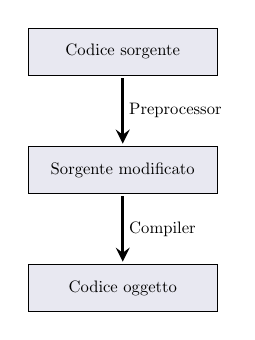
\begin{tikzpicture}[scale=0.6, every node/.style={scale=0.6}]
    \filldraw[fill=MidnightBlue!10!white] (0,0) rectangle ++(4,1);
    \filldraw[fill=MidnightBlue!10!white] (0,-2.5) rectangle ++(4,1);
    \filldraw[fill=MidnightBlue!10!white] (0,-5) rectangle ++(4,1);
    \path (2,0.5) node {Codice sorgente}
          (2,-2) node {Sorgente modificato}
          (2,-4.5) node {Codice oggetto};
    \draw[-stealth,very thick,shorten >=1pt,shorten <=1pt] (2,0) -- node[right] {Preprocessor} (2,-1.5);
    \draw[-stealth,very thick,shorten >=1pt,shorten <=1pt] (2,-2.5) -- node[right] {Compiler} (2,-4);
  \end{tikzpicture}\end{center}
  \vfill
  \begin{itemize}
    \item Il codice sorgente viene scritto per intero \vfill
    \item Il \alert{preprocessor} modifica al sorgente (facoltativo) \vfill
    \item Il \alert{compiler} crea un file oggetto dal sorgente
  \end{itemize}
  \vfill
\end{frame}

\begin{frame}{Linguaggi interpretati}
  \vfill
  \begin{center}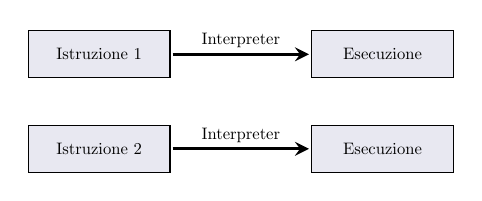
\begin{tikzpicture}[scale=0.6, every node/.style={scale=0.6}]
    \filldraw[fill=MidnightBlue!10!white] (0,0) rectangle ++(3,1);
    \filldraw[fill=MidnightBlue!10!white] (6,0) rectangle ++(3,1);
    \path (1.5,0.5) node {Istruzione 1};
    \path (7.5,0.5) node {Esecuzione};
    \draw[-stealth,very thick,shorten >=1pt,shorten <=1pt] (3,0.5) -- node[above] {Interpreter} (6,0.5);
    \begin{scope}[shift={(0,-2)}]
      \filldraw[fill=MidnightBlue!10!white] (0,0) rectangle ++(3,1);
      \filldraw[fill=MidnightBlue!10!white] (6,0) rectangle ++(3,1);
      \path (1.5,0.5) node {Istruzione 2};
      \path (7.5,0.5) node {Esecuzione};
      \draw[-stealth,very thick,shorten >=1pt,shorten <=1pt] (3,0.5) -- node[above] {Interpreter} (6,0.5);
    \end{scope}
  \end{tikzpicture}\end{center}
  \vfill
  \begin{itemize}
    \item Ciascuna istruzione viene compilata singolarmente
    \vfill
    \item Esecuzione di programm incompleti
    \vfill
    \item Molto più lenti dei linguaggi compilati
  \end{itemize}
  \vfill
\end{frame}

\begin{frame}{Paradigmi}
  \vfill
  \begin{itemize}
    \item Programmazione imperativa
    \begin{itemize}
      \item lista di \alert{comandi} eseguiti in un certo ordine
    \end{itemize}
    \vfill
    \item Programmazione dichiarativa
    \begin{itemize}
      \item lista di \alert{relazioni} tra enti
    \end{itemize}
    \vfill
    \item Programmazione ad oggetti
    \begin{itemize}
      \item lista di \alert{oggetti} e di \alert{interazioni} tra essi
    \end{itemize}
  \end{itemize}
  \vfill
\end{frame}

\begin{frame}{Programmazione imperativa}
  \vfill
  \begin{itemize}
    \item Scrittura di un \alert{algoritmo} per risolvere un problema
    \vfill
    \item Esempio: cambiare la batteria di un telecomando
    \begin{itemize}
      \item aprire il vano batterie
      \item rimuovere la vecchia batteria
      \item gettare la vecchia batteria
      \item inserire la nuova batteria
      \item chiudere il vano batterie
    \end{itemize}
    \vfill
    \item L'ordine delle istruzioni è determinante
  \end{itemize}
  \vfill
\end{frame}

\begin{frame}{Flowcharts}
  \vfill
  \begin{itemize}
    \item Per rappresentare un algoritmo si utilizzano i \alert{flowcharts} o \alert{diagrammi di flusso}
    \vfill
    \item Un flowchart è costituito da
    \begin{itemize}
      \item celle contenenti istruzioni
      \item frecce che guidano il \alert{flusso di controllo}
    \end{itemize}
    \vfill
    \item I flowcharts sono un linguaggio di programmazione
    \vfill
    \item Creare flowcharts aiuta nella stesura di un algoritmo
  \end{itemize}
  \vfill
\end{frame}

\begin{frame}{Flowcharts}
  \vfill
  \begin{center}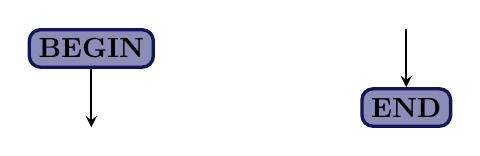
\begin{tikzpicture}[node distance=15mm]
  \node[begin] (start) at (0,0) {\textbf{BEGIN}};
  \draw[arrow] (start) to ++(0,-1);
  \node[begin] (end) at (4,-0.75) {\textbf{END}};
  \draw[arrow] (4,0.25) to (end);
  \end{tikzpicture}\end{center}
  \vfill
  \begin{itemize}
    \item Istruzioni di inizio e fine diagramma
    \vfill
    \item Uno ed un solo \alert{BEGIN} per diagramma
    \vfill
    \item A volte ammessi più \alert{END} in un singolo diagramma
  \end{itemize}
\end{frame}

\begin{frame}{Flowcharts}
  \vfill
  \begin{center}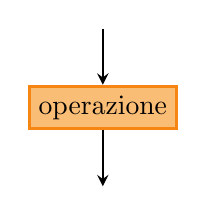
\begin{tikzpicture}[node distance=15mm]
  \node[operation] (op) at (0,0) {operazione};
  \draw[arrow] (op) to ++(0,-1);
  \draw[arrow] (0,1) to (op);
  \end{tikzpicture}\end{center}
  \vfill
  \begin{itemize}
    \item Istruzione di processo
    \vfill
    \item Viene eseguita l'operazione indicata nella casella
  \end{itemize}
\end{frame}

\begin{frame}{Flowcharts}
  \vfill
  \begin{center}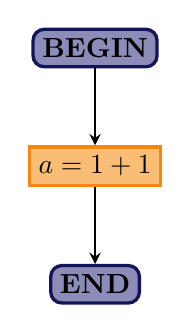
\begin{tikzpicture}[node distance=15mm]
    \node[begin] (start) {\textbf{BEGIN}};
    \node[below of=start,operation](init){\(a = 1+1\)};
    \node[below of=init,begin](end){\textbf{END}};

    \draw[arrow] (start) to (init);
    \draw[arrow] (init) to (end);
  \end{tikzpicture}\end{center}
  \vfill
  \begin{itemize}
    \item Il programma calcola 1+1 \vfill
    \item Il risultato viene messo nella \alert{variabile} \(a\)
  \end{itemize}
\end{frame}

\begin{frame}{Flowcharts}
  \vfill
  \begin{center}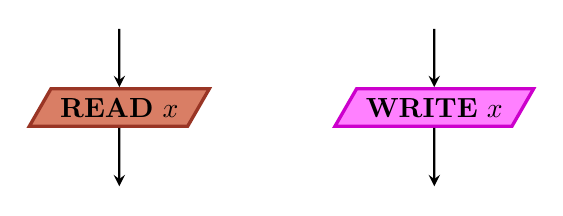
\begin{tikzpicture}[node distance=15mm]
  \node[input] (in) at (0,0) {\textbf{READ} \(x\)};
  \draw[arrow] (in) to ++(0,-1);
  \draw[arrow] (0,1) to (in);
  \node[output] (out) at (4,0) {\textbf{WRITE} \(x\)};
  \draw[arrow] (out) to ++(0,-1);
  \draw[arrow] (4,1) to (out);
  \end{tikzpicture}\end{center}
  \vfill
  \begin{itemize}
    \item Istruzioni di lettura/scrittura
    \vfill
    \item Lettura: un valore inserito dall'\alert{utente} viene memorizzato nella
    variabile \(x\)
    \vfill
    \item Scrittura: il valore corrente della variabile \(x\) viene comunicato all'\alert{utente}
  \end{itemize}
\end{frame}

\begin{frame}{Flowcharts}
  \vfill
  \begin{center}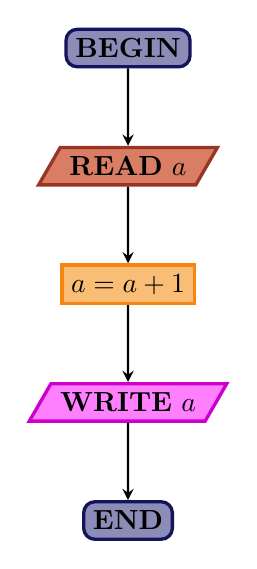
\begin{tikzpicture}[node distance=15mm]
    \node[begin] (start) {\textbf{BEGIN}};
    \node[below of=start,input](in){\textbf{READ} \(a\)};
    \node[below of=in,operation](op){\(a = a+1\)};
    \node[below of=op,output](out){\textbf{WRITE} \(a\)};
    \node[below of=out,begin](end){\textbf{END}};

    \draw[arrow] (start) to (in);
    \draw[arrow] (in) to (op);
    \draw[arrow] (op) to (out);
    \draw[arrow] (out) to (end);
  \end{tikzpicture}\end{center}
  \vfill
\end{frame}

\begin{frame}{Flowcharts}
  \vfill
  \begin{center}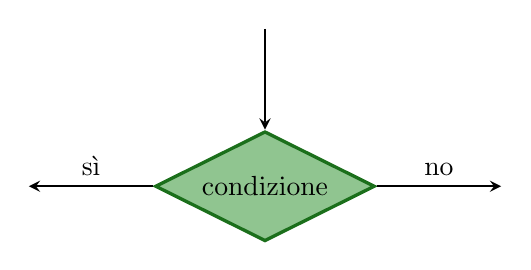
\begin{tikzpicture}[node distance=15mm]
  \node[decision] (op) at (0,0) {condizione};
  \draw[arrow] (op) to node[above]{no} ++(3,0);
  \draw[arrow] (op) to node[above]{sì} ++(-3,0);
  \draw[arrow] (0,2) to (op);
  \end{tikzpicture}\end{center}
  \vfill
  \begin{itemize}
    \item Istruzione condizionale
    \vfill
    \item Il flusso del grafico cambia direzione a seconda che la condizione
    sia vera oppure falsa
  \end{itemize}
\end{frame}

\begin{frame}{Flowcharts}
  \vfill
  \begin{center}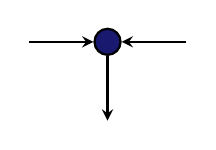
\begin{tikzpicture}[node distance=15mm]
  \node[connection] (cn) at (0,0) {};
  \draw[arrow] (cn) to ++(0,-1);
  \draw[arrow] (-1,0) to (cn);
  \draw[arrow] (1,0) to (cn);
  \end{tikzpicture}\end{center}
  \vfill
  \begin{itemize}
    \item Connettore
    \vfill
    \item Permette di rincongiungere due rami separati
  \end{itemize}
\end{frame}

\begin{frame}{Flowcharts}
  \vfill
  \begin{center}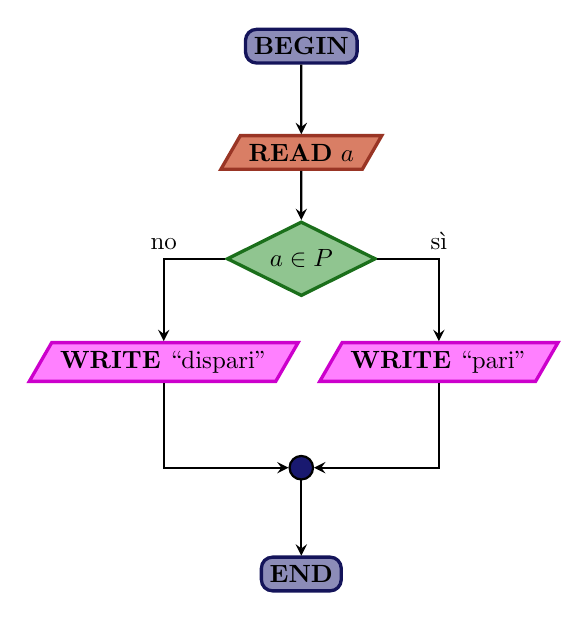
\begin{tikzpicture}[scale=0.9, every node/.style={scale=0.9},node distance=15mm]
    \node[begin] (start) {\textbf{BEGIN}};
    \node[below of=start,input](in){\textbf{READ} \(a\)};
    \node[below of=in,decision](dec){\(a \in \mathbb{P}\)};
    \node[below right = 8mm and 10mm of dec,output](pari){\textbf{WRITE} ``pari''};
    \node[below left = 8mm and 10mm of dec,output](dispari){\textbf{WRITE} ``dispari''};
    \node[below = 20mm of dec,connection](conn){};
    \node[below of=conn,begin](end){\textbf{END}};

    \draw[arrow] (start) to (in);
    \draw[arrow] (in) to (dec);
    \draw[arrow] (dec) -| node[above] {no} (dispari);
    \draw[arrow] (dec) -| node[above] {sì} (pari);
    \draw[arrow] (dispari) |- (conn);
    \draw[arrow] (pari) |- (conn);
    \draw[arrow] (conn) to (end);
  \end{tikzpicture}\end{center}
  \vfill
\end{frame}

\begin{frame}{Flowcharts}
  \vfill
  \begin{itemize}
    \item Le regole elencate danno origine alla programmazione imperativa in senso lato
    \vfill
    \item Le frecce possono ``risalire'' il diagramma
    \begin{itemize}
      \item istruzioni \alert{goto}: ritorno ad un punto precedente
    \end{itemize}
    \vfill
    \item Questo rende più difficile:
    \begin{itemize}
      \item studio formale del programma
      \item apportare modifiche al codice
      \item comprensione del programma da parte di terzi
    \end{itemize}
  \end{itemize}
\end{frame}

\begin{frame}{Flowcharts}
  \vfill
  \begin{itemize}
    \item La programmazione \alert{strutturata} vieta i goto
    \vfill
    \item Le frecce non possono risalire il diagramma
    \vfill
    \item Viene aggiunto un nuovo simbolo
    \vfill
    \item Teorema di Böhm-Jacopini
    \begin{itemize}
      \item \alert{equivalenza} tra imperativa e strutturata
    \end{itemize}
  \end{itemize}
\end{frame}

\begin{frame}{Flowcharts}
  \vfill
  \begin{center}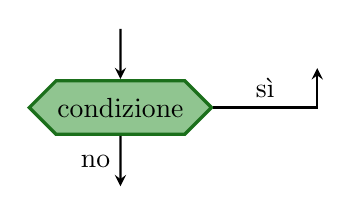
\begin{tikzpicture}[node distance=15mm]
  \node[loop] (op) at (0,0) {condizione};
  \draw[arrow] (op) to node[left]{no} ++(0,-1);
  \draw[arrow] (op) to node[above]{sì} ++(2.5,0) to ++(0,.5);
  \draw[arrow] (0,1) to (op);
  \end{tikzpicture}\end{center}
  \vfill
  \begin{itemize}
    \item Istruzione di loop
    \vfill
    \item Concettualmente identica all'istruzione condizionale, ma uno (ed uno solo)
    dei due flussi può risalire
    \vfill
    \item Permette di ripetere una serie di istruzioni
  \end{itemize}
\end{frame}

\begin{frame}{Flowcharts}
  \vfill
  \begin{center}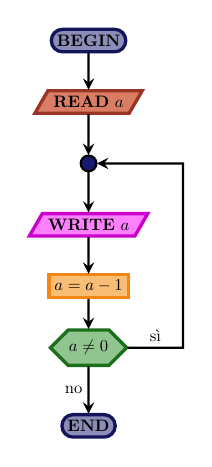
\begin{tikzpicture}[scale=0.6, every node/.style={scale=0.6},node distance=13mm]
    \node[begin] (start) {\textbf{BEGIN}};
    \node[below of=start,input] (read) {\textbf{READ} \(a\)};
    \node[below of=read,connection] (conn) {};
    \node[below of=conn,output] (write) {\textbf{WRITE} \(a\)};
    \node[below of=write,operation](decr){\(a = a-1\)};
    \node[below of=decr,loop](loop){\(a \neq 0\)};
    \node[below = 6mm of loop,begin](end){\textbf{END}};

    \draw[arrow] (start) to (read);
    \draw[arrow] (read) to (conn);
    \draw[arrow] (conn) to (write);
    \draw[arrow] (write) to (decr);
    \draw[arrow] (decr) to (loop);
    \draw[arrow] (loop) to node[anchor=east]{no} (end);
    \draw[arrow] (loop) to node[anchor=south]{sì} ++(20mm,0) |- (conn);
  \end{tikzpicture}\end{center}
  \vfill
\end{frame}

\begin{frame}{Flowcharts}
  \vfill
  \begin{center}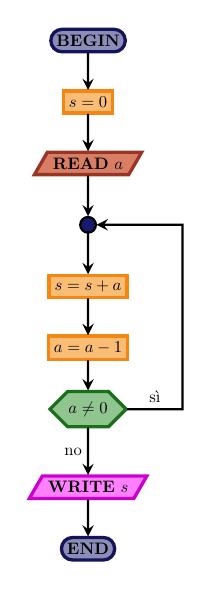
\begin{tikzpicture}[scale=0.6, every node/.style={scale=0.6},node distance=13mm]
    \node[begin] (start) {\textbf{BEGIN}};
    \node[below of=start,operation](init){\(s = 0\)};
    \node[below of=init,input] (read) {\textbf{READ} \(a\)};
    \node[below of=read,connection] (conn) {};
    \node[below of=conn,operation](add){\(s = s+a\)};
    \node[below of=add,operation](decr){\(a = a-1\)};
    \node[below of=decr,loop](loop){\(a \neq 0\)};
    \node[below = 6mm of loop,output] (write) {\textbf{WRITE} \(s\)};
    \node[below of=write,begin](end){\textbf{END}};

    \draw[arrow] (start) to (init);
    \draw[arrow] (init) to (read);
    \draw[arrow] (read) to (conn);
    \draw[arrow] (conn) to (add);
    \draw[arrow] (add) to (decr);
    \draw[arrow] (decr) to (loop);
    \draw[arrow] (loop) to node[anchor=east]{no} (write);
    \draw[arrow] (loop) to node[anchor=south]{sì} ++(20mm,0) |- (conn);
  \draw[arrow] (write) to (end);
  \end{tikzpicture}\end{center}
  \vfill
\end{frame}

\begin{frame}[fragile]{Hello, World!}
  \vfill
  \begin{center}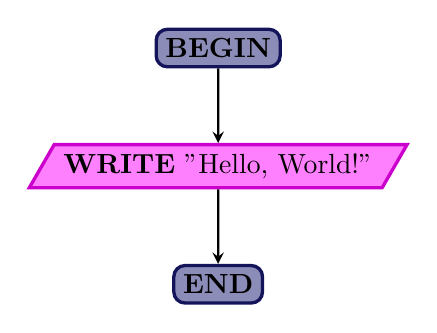
\begin{tikzpicture}[node distance=15mm]
    \node[begin] (start) {\textbf{BEGIN}};
    \node[below of=start,output](init){\textbf{WRITE} "Hello, World!"};
    \node[below of=init,begin](end){\textbf{END}};

    \draw[arrow] (start) to (init);
    \draw[arrow] (init) to (end);
  \end{tikzpicture}\end{center}
  \vfill
  \begin{lstlisting}
#include <iostream>

int main() {
  std::cout << "Hello, World!" << std::endl;
  return 0;
}
  \end{lstlisting}
  \vfill
\end{frame}

\begin{frame}[fragile]{Hello, World!}
  \vfill
  \begin{itemize}
    \item Il codice sorgente viene scritto in un file di testo
    \begin{itemize}
      \item estensioni standard \lstinline$*.cpp$ o \lstinline$*.cc$ o \lstinline$*.C$
    \end{itemize}
    \vfill
    \item La compilazione può avvenire in due modi
    \begin{itemize}
      \item tramite IDE (ambiente di sviluppo)
      \item \lstinline$g++ -std=c++14 source.cpp -o target$
    \end{itemize}
    \vfill
    \item Per progetti più ampi conviene creare un \alert{Makefile}
  \end{itemize}
  \vfill
\end{frame}

\begin{frame}[fragile]{Hello, World!}
  \vfill
  \begin{lstlisting}
#include <iostream>

int main() {
  std::cout << "Hello, World!" << std::endl;
  return 0;
}
  \end{lstlisting}
  \vfill
  \begin{itemize}
    \item \lstinline$#$ introduce direttive del preprocessore
    \vfill
    \item \lstinline$int main()$ è la parte principale del programma
    \vfill
    \item \lstinline${ ... }$ raggruppa più istruzioni in un singolo blocco
    \vfill
    \item ogni istruzione termina con un \lstinline$;$
    \vfill
    \item ogni programma deve terminare con \lstinline$return 0;$
    \vfill
    \item l'ultima riga di un file deve sempre essere vuota
  \end{itemize}
  \vfill
\end{frame}

\begin{frame}[fragile]{Hello, World!}
  \vfill
  \begin{lstlisting}
#include <iostream>

int main() {
  std::cout << "Hello, World!" << std::endl;
  return 0;
}
  \end{lstlisting}
  \vfill
  \begin{itemize}
    \item \lstinline$#include <...>$ inserisce un \alert{header} nel programma
    \begin{itemize}
      \item funzioni di libreria (C++ Standard Library)
      \item tutte nel \alert{namespace} \lstinline$std$
    \end{itemize}
    \vfill
    \item \lstinline$<iostream>$ contiene:
    \begin{itemize}
      \item \lstinline$std::cout$ necessaria per scrivere a schermo
      \item \lstinline$std::endl$ inserisce un'interruzione di riga
    \end{itemize}
  \end{itemize}
  \vfill
\end{frame}

\begin{frame}[fragile]{Hello, World!}
  \vfill
  \begin{lstlisting}
#include <iostream>

int main() {
  std::cout << "Hello, World!" << std::endl;
  return 0;
}
  \end{lstlisting}
  \vfill
  \begin{itemize}
    \item C++ gestisce l'output tramite \alert{stream} (flussi)
    \begin{itemize}
      \item \lstinline$std::cout$ è il flusso di output standard
      \item \lstinline$<<$ è l'operatore di \alert{inserimento}
      \item \lstinline$std::endl$ è un \alert{manipolatore}
    \end{itemize}
    \vfill
    \item \lstinline$"Hello, World!"$ è una \alert{stringa}
    \begin{itemize}
      \item delimitate da \alert{virgolette}
    \end{itemize}
  \end{itemize}
  \vfill
\end{frame}

\begin{frame}[fragile]{Hello, World!}
  \vfill
  \begin{lstlisting}
//Questo è il mio primo programma in C++
#include <iostream>

int main() {
  std::cout << "Hello, World!" << std::endl;
  return 0;
}
  \end{lstlisting}
  \vfill
  \begin{itemize}
    \item le righe introdotte da \lstinline$//$ sono \alert{commenti}
    \vfill
    \item commentare è una buona abitudine
    \begin{itemize}
      \item aiuta a ricordare cosa fa il programma
      \item aiuta altri a capire cosa fa il programma
    \end{itemize}
    \vfill
    \item altro modo di creare commenti: \lstinline$/* ... */$
  \end{itemize}
  \vfill
\end{frame}

\begin{frame}[fragile]{Hello, World!}
  \vfill
  \begin{lstlisting}
//Questo è il mio primo programma in C++
#include <iostream>
using namespace std;
int main() {
  cout << "Hello, World!" << endl;
  return 0;
}
  \end{lstlisting}
  \vfill
  \begin{itemize}
    \item Importa \alert{tutte} le funzioni del namespace std
    \vfill
    \item Comodo per non scrivere \lstinline$std::$ ogni volta
    \vfill
    \item Cattiva abitudine, molto rischioso
  \end{itemize}
  \vfill
\end{frame}

\begin{frame}[fragile]{Hello, World!}
  \vfill
  \begin{lstlisting}
//Questo è il mio primo programma in C++
#include <iostream>
using std::cout;
using std::endl;
int main() {
  cout << "Hello, World!" << endl;
  return 0;
}
  \end{lstlisting}
  \vfill
  \begin{itemize}
    \item Importa soltanto le funzioni che richiediamo
    \vfill
    \item Più sicuro che importare l'intero namespace
  \end{itemize}
  \vfill
\end{frame}

\begin{frame}[fragile]{Variabili}
  \vfill
  \begin{columns}[c]
    \column{.45\textwidth}
    \vfill
    \begin{lstlisting}
#include <iostream>
using std::cout;
using std::endl;
int main() {
  int a;
  a = 5;
  cout << a << endl;
  return 0;
}
    \end{lstlisting}
    \vfill
    \column{.45\textwidth}
    \vfill
    \begin{center}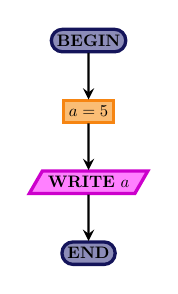
\begin{tikzpicture}[node distance=15mm, scale=0.6, every node/.style={scale=0.6}]
      \node[begin] (start) {\textbf{BEGIN}};
      \node[below of=start,operation](op){\(a = 5\)};
      \node[below of=op,output](out){\textbf{WRITE} \(a\)};
      \node[below of=out,begin](end){\textbf{END}};

      \draw[arrow] (start) to (op);
      \draw[arrow] (op) to (out);
      \draw[arrow] (out) to (end);
    \end{tikzpicture}\end{center}
    \vfill
  \end{columns}
  \vfill
  \begin{itemize}
    \item \lstinline$int a;$ \alert{dichiara} la variabile \lstinline$a$ di \alert{tipo} \lstinline$int$
    \vfill
    \item \lstinline$a = 5;$ \alert{assegna} il valore \lstinline$5$ alla variabile \lstinline$a$
    \begin{itemize}
      \item la prima assegnazione è detta \alert{inizializzazione}
      \item \alert{mai} utilizzare una variabile non inizializzata
    \end{itemize}
  \end{itemize}
  \vfill
\end{frame}

\begin{frame}[fragile]{Variabili}
  \vfill
  \begin{columns}[c]
    \column{.45\textwidth}
    \vfill
    \begin{lstlisting}
#include <iostream>
using std::cout;
using std::endl;
int a;
int main() {
  a = 5;
  cout << a << endl;
  return 0;
}
    \end{lstlisting}
    \vfill
    \column{.45\textwidth}
    \vfill
    \begin{center}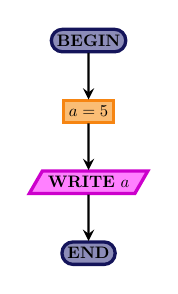
\begin{tikzpicture}[node distance=15mm, scale=0.6, every node/.style={scale=0.6}]
      \node[begin] (start) {\textbf{BEGIN}};
      \node[below of=start,operation](op){\(a = 5\)};
      \node[below of=op,output](out){\textbf{WRITE} \(a\)};
      \node[below of=out,begin](end){\textbf{END}};

      \draw[arrow] (start) to (op);
      \draw[arrow] (op) to (out);
      \draw[arrow] (out) to (end);
    \end{tikzpicture}\end{center}
    \vfill
  \end{columns}
  \vfill
  \begin{itemize}
    \item Dichiarazione all'esterno di \lstinline$main()$
    \vfill
    \item Variabile \alert{globale}
    \vfill
    \item Ammesso, ma fortemente sconsigliato
  \end{itemize}
  \vfill
\end{frame}

\begin{frame}[fragile]{Variabili}
  \vfill
  \begin{columns}[c]
    \column{.45\textwidth}
    \vfill
    \begin{lstlisting}
#include <iostream>
using std::cout;
using std::endl;
int main() {
  int a = 5;
  cout << a << endl;
  return 0;
}
    \end{lstlisting}
    \vfill
    \column{.45\textwidth}
    \vfill
    \begin{center}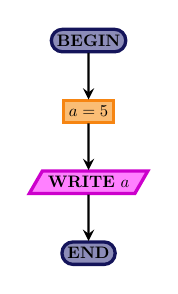
\begin{tikzpicture}[node distance=15mm, scale=0.6, every node/.style={scale=0.6}]
      \node[begin] (start) {\textbf{BEGIN}};
      \node[below of=start,operation](op){\(a = 5\)};
      \node[below of=op,output](out){\textbf{WRITE} \(a\)};
      \node[below of=out,begin](end){\textbf{END}};

      \draw[arrow] (start) to (op);
      \draw[arrow] (op) to (out);
      \draw[arrow] (out) to (end);
    \end{tikzpicture}\end{center}
    \vfill
  \end{columns}
  \vfill
  \begin{itemize}
    \item Inizializzazione in sede di dichiarazione
    \vfill
    \item Buona abitudine
  \end{itemize}
  \vfill
\end{frame}

\begin{frame}[fragile]{Variabili}
  \vfill
  \begin{columns}[c]
    \column{.45\textwidth}
    \vfill
    \begin{lstlisting}
#include <iostream>
using std::cout;
using std::endl;
int main() {
  int a;
  a = 5 + 2;
  cout << a << endl;
  return 0;
}
    \end{lstlisting}
    \vfill
    \column{.45\textwidth}
    \vfill
    \begin{center}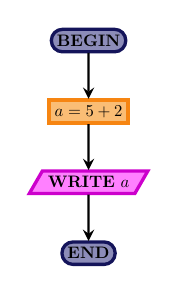
\begin{tikzpicture}[node distance=15mm, scale=0.6, every node/.style={scale=0.6}]
      \node[begin] (start) {\textbf{BEGIN}};
      \node[below of=start,operation](op){\(a = 5 + 2\)};
      \node[below of=op,output](out){\textbf{WRITE} \(a\)};
      \node[below of=out,begin](end){\textbf{END}};

      \draw[arrow] (start) to (op);
      \draw[arrow] (op) to (out);
      \draw[arrow] (out) to (end);
    \end{tikzpicture}\end{center}
    \vfill
  \end{columns}
  \vfill
  \begin{itemize}
    \item È possibile compiere operazioni
  \end{itemize}
  \vfill
\end{frame}

\begin{frame}[fragile]{Variabili}
  \vfill
  \begin{columns}[c]
    \column{.45\textwidth}
    \vfill
    \begin{lstlisting}
#include <iostream>
using std::cout;
using std::endl;
int main() {
  int a = 5;
  a = a + 2;
  cout << a << endl;
  return 0;
}
    \end{lstlisting}
    \vfill
    \column{.45\textwidth}
    \vfill
    \begin{center}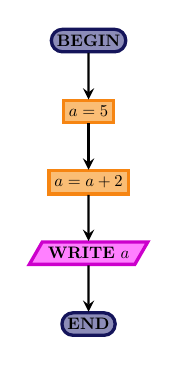
\begin{tikzpicture}[node distance=15mm, scale=0.6, every node/.style={scale=0.6}]
      \node[begin] (start) {\textbf{BEGIN}};
      \node[below of=start,operation](op1){\(a = 5\)};
      \node[below of=op1,operation](op2){\(a = a + 2\)};
      \node[below of=op2,output](out){\textbf{WRITE} \(a\)};
      \node[below of=out,begin](end){\textbf{END}};

      \draw[arrow] (start) to (op1);
      \draw[arrow] (op1) to (op2);
      \draw[arrow] (op2) to (out);
      \draw[arrow] (out) to (end);
    \end{tikzpicture}\end{center}
    \vfill
  \end{columns}
  \vfill
  \begin{itemize}
    \item Utilizzo del valore di una variabile in un'operazione:
    \begin{itemize}
      \item leggo il valore di \lstinline$a$
      \item sommo \lstinline$2$ al valore letto
      \item metto il risultato in \lstinline$a$
    \end{itemize}
  \end{itemize}
  \vfill
\end{frame}

\begin{frame}[fragile]{Variabili}
  \vfill
  \begin{columns}[c]
    \column{.45\textwidth}
    \vfill
    \begin{lstlisting}
#include <iostream>
using std::cout;
using std::endl;
int main() {
  int a = 5;
  a += 2;
  cout << a << endl;
  return 0;
}
    \end{lstlisting}
    \vfill
    \column{.45\textwidth}
    \vfill
    \begin{center}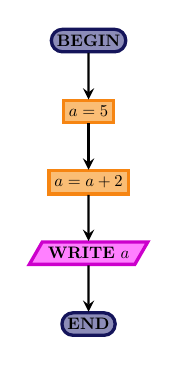
\begin{tikzpicture}[node distance=15mm, scale=0.6, every node/.style={scale=0.6}]
      \node[begin] (start) {\textbf{BEGIN}};
      \node[below of=start,operation](op1){\(a = 5\)};
      \node[below of=op1,operation](op2){\(a = a + 2\)};
      \node[below of=op2,output](out){\textbf{WRITE} \(a\)};
      \node[below of=out,begin](end){\textbf{END}};

      \draw[arrow] (start) to (op1);
      \draw[arrow] (op1) to (op2);
      \draw[arrow] (op2) to (out);
      \draw[arrow] (out) to (end);
    \end{tikzpicture}\end{center}
    \vfill
  \end{columns}
  \vfill
  \begin{itemize}
    \item Forma più compatta della scrittura precedente
  \end{itemize}
  \vfill
\end{frame}

\begin{frame}[fragile]{Variabili}
  \vfill
  \begin{itemize}
    \item Operazioni:\\[.5em]
    \hspace{5mm}\begin{tabular}{cll}
      \lstinline$+$ & somma & \lstinline$5 + 3 = 8$ \\
      \lstinline$-$ & sottrazione & \lstinline$5 - 3 = 2$ \\
      \lstinline$*$ & moltiplicazione & \lstinline$5 * 3 = 15$ \\
      \lstinline$/$ & divisione & \lstinline$5 / 3 = 1$ \\
      \lstinline!%! & resto & \lstinline!5 % 3 = 2! \\
    \end{tabular}
  \end{itemize}
  \vfill
\end{frame}

\begin{frame}[fragile]{Variabili}
  \vfill
  \begin{columns}[c]
    \column{.45\textwidth}
    \vfill
    \begin{lstlisting}
#include <iostream>
using std::cout;
using std::endl;
int main() {
  int a;
  int b;
  a = 5;
  b = 3;
  cout << a << endl;
  cout << b << endl;
  return 0;
}
    \end{lstlisting}
    \vfill
    \column{.45\textwidth}
    \vfill
    \begin{center}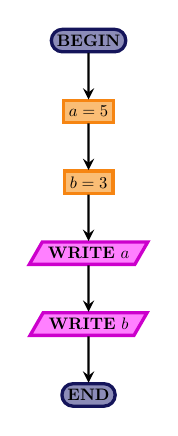
\begin{tikzpicture}[node distance=15mm, scale=0.6, every node/.style={scale=0.6}]
      \node[begin] (start) {\textbf{BEGIN}};
      \node[below of=start,operation](op1){\(a = 5\)};
      \node[below of=op1,operation](op2){\(b = 3\)};
      \node[below of=op2,output](out1){\textbf{WRITE} \(a\)};
      \node[below of=out1,output](out2){\textbf{WRITE} \(b\)};
      \node[below of=out2,begin](end){\textbf{END}};

      \draw[arrow] (start) to (op1);
      \draw[arrow] (op1) to (op2);
      \draw[arrow] (op2) to (out1);
      \draw[arrow] (out1) to (out2);
      \draw[arrow] (out2) to (end);
    \end{tikzpicture}\end{center}
    \vfill
  \end{columns}
  \vfill
  \begin{itemize}
    \item Posso dichiarare più variabili
  \end{itemize}
  \vfill
\end{frame}

\begin{frame}[fragile]{Variabili}
  \vfill
  \begin{columns}[c]
    \column{.45\textwidth}
    \vfill
    \begin{lstlisting}
#include <iostream>
using std::cout;
using std::endl;
int main() {
  int a, b;
  a = 5;
  b = 3;
  cout << a << endl;
  cout << b << endl;
  return 0;
}
    \end{lstlisting}
    \vfill
    \column{.45\textwidth}
    \vfill
    \begin{center}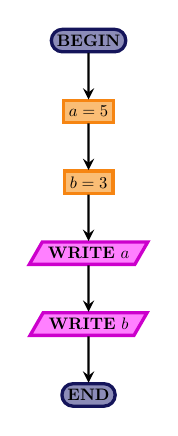
\begin{tikzpicture}[node distance=15mm, scale=0.6, every node/.style={scale=0.6}]
      \node[begin] (start) {\textbf{BEGIN}};
      \node[below of=start,operation](op1){\(a = 5\)};
      \node[below of=op1,operation](op2){\(b = 3\)};
      \node[below of=op2,output](out1){\textbf{WRITE} \(a\)};
      \node[below of=out1,output](out2){\textbf{WRITE} \(b\)};
      \node[below of=out2,begin](end){\textbf{END}};

      \draw[arrow] (start) to (op1);
      \draw[arrow] (op1) to (op2);
      \draw[arrow] (op2) to (out1);
      \draw[arrow] (out1) to (out2);
      \draw[arrow] (out2) to (end);
    \end{tikzpicture}\end{center}
    \vfill
  \end{columns}
  \vfill
  \begin{itemize}
    \item Variabili dello stesso tipo possono essere dichiarate in un'unica istruzione,
    separate da virgole
  \end{itemize}
  \vfill
\end{frame}

\begin{frame}[fragile]{Variabili}
  \vfill
  \begin{columns}[c]
    \column{.45\textwidth}
    \vfill
    \begin{lstlisting}
#include <iostream>
using std::cout;
using std::endl;
int main() {
  int a = 5, b = 3;
  cout << a << endl;
  cout << b << endl;
  return 0;
}
    \end{lstlisting}
    \vfill
    \column{.45\textwidth}
    \vfill
    \begin{center}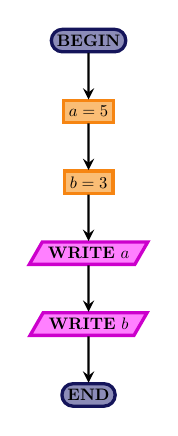
\begin{tikzpicture}[node distance=15mm, scale=0.6, every node/.style={scale=0.6}]
      \node[begin] (start) {\textbf{BEGIN}};
      \node[below of=start,operation](op1){\(a = 5\)};
      \node[below of=op1,operation](op2){\(b = 3\)};
      \node[below of=op2,output](out1){\textbf{WRITE} \(a\)};
      \node[below of=out1,output](out2){\textbf{WRITE} \(b\)};
      \node[below of=out2,begin](end){\textbf{END}};

      \draw[arrow] (start) to (op1);
      \draw[arrow] (op1) to (op2);
      \draw[arrow] (op2) to (out1);
      \draw[arrow] (out1) to (out2);
      \draw[arrow] (out2) to (end);
    \end{tikzpicture}\end{center}
    \vfill
  \end{columns}
  \vfill
  \begin{itemize}
    \item Inizializzazione in sede di dichiarazione
  \end{itemize}
  \vfill
\end{frame}

\begin{frame}[fragile]{Variabili}
  \vfill
  \begin{columns}[c]
    \column{.45\textwidth}
    \vfill
    \begin{lstlisting}
#include <iostream>
using std::cout;
using std::endl;
int main() {
  int a = 5, b;
  b = a++;
  cout << a << endl;
  cout << b << endl;
  return 0;
}
    \end{lstlisting}
    \vfill
    \column{.45\textwidth}
    \vfill
    \begin{center}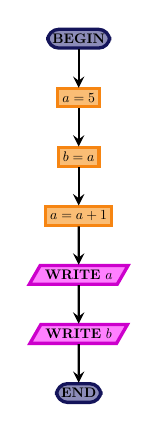
\begin{tikzpicture}[node distance=15mm, scale=0.5, every node/.style={scale=0.5}]
      \node[begin] (start) {\textbf{BEGIN}};
      \node[below of=start,operation](op1){\(a = 5\)};
      \node[below of=op1,operation](op2){\(b = a\)};
      \node[below of=op2,operation](op3){\(a = a + 1\)};
      \node[below of=op3,output](out1){\textbf{WRITE} \(a\)};
      \node[below of=out1,output](out2){\textbf{WRITE} \(b\)};
      \node[below of=out2,begin](end){\textbf{END}};

      \draw[arrow] (start) to (op1);
      \draw[arrow] (op1) to (op2);
      \draw[arrow] (op2) to (op3);
      \draw[arrow] (op3) to (out1);
      \draw[arrow] (out1) to (out2);
      \draw[arrow] (out2) to (end);
    \end{tikzpicture}\end{center}
    \vfill
  \end{columns}
  \vfill
  \begin{itemize}
    \item \lstinline$a++$ operatore di \alert{post-incremento}
    \vfill
    \item \lstinline$a--$ operatore di \alert{post-decremento}
  \end{itemize}
  \vfill
\end{frame}

\begin{frame}[fragile]{Variabili}
  \vfill
  \begin{columns}[c]
    \column{.45\textwidth}
    \vfill
    \begin{lstlisting}
#include <iostream>
using std::cout;
using std::endl;
int main() {
  int a = 5, b;
  b = ++a;
  cout << a << endl;
  cout << b << endl;
  return 0;
}
    \end{lstlisting}
    \vfill
    \column{.45\textwidth}
    \vfill
    \begin{center}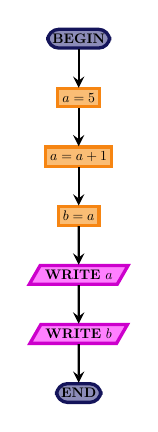
\begin{tikzpicture}[node distance=15mm, scale=0.5, every node/.style={scale=0.5}]
      \node[begin] (start) {\textbf{BEGIN}};
      \node[below of=start,operation](op1){\(a = 5\)};
      \node[below of=op1,operation](op2){\(a = a + 1\)};
      \node[below of=op2,operation](op3){\(b = a\)};
      \node[below of=op3,output](out1){\textbf{WRITE} \(a\)};
      \node[below of=out1,output](out2){\textbf{WRITE} \(b\)};
      \node[below of=out2,begin](end){\textbf{END}};

      \draw[arrow] (start) to (op1);
      \draw[arrow] (op1) to (op2);
      \draw[arrow] (op2) to (op3);
      \draw[arrow] (op3) to (out1);
      \draw[arrow] (out1) to (out2);
      \draw[arrow] (out2) to (end);
    \end{tikzpicture}\end{center}
    \vfill
  \end{columns}
  \vfill
  \begin{itemize}
    \item \lstinline$++a$ operatore di \alert{pre-incremento}
    \vfill
    \item \lstinline$--a$ operatore di \alert{pre-decremento}
  \end{itemize}
  \vfill
\end{frame}

\begin{frame}[fragile]{Variabili}
  \vfill
  \begin{itemize}
    \item Tipi di variabile:
    \begin{itemize}
      \item numeri interi
      \begin{itemize}
          \item \lstinline$short$
          \item \lstinline$int$
          \item \lstinline$long$
          \item \lstinline$long long$
      \end{itemize}
        \item numeri interi
        \begin{itemize}
            \item \lstinline$float$
            \item \lstinline$double$
            \item \lstinline$long double$
        \end{itemize}
      \item booleano (0/1)
      \begin{itemize}
        \item \lstinline$bool$
      \end{itemize}
      \item carattere
      \begin{itemize}
        \item \lstinline$char$
      \end{itemize}
    \end{itemize}
  \end{itemize}
  \vfill
\end{frame}

\begin{frame}[fragile]{Variabili}
  \vfill
  \begin{lstlisting}
#include <iostream>
#include <limits>
using std::cout;
using std::endl;
int main() {
  cout << std::numeric_limits<int>::max() << endl;
  cout << std::numeric_limits<int>::min() << endl;
  return 0;
}
  \end{lstlisting}
  \vfill
  \begin{itemize}
    \item La dimensione dei tipi non è standard
    \vfill
    \item Ogni compilatore può avere dimensioni diverse
    \vfill
    \item È bene verificare i limiti del proprio compilatore
  \end{itemize}
  \vfill
\end{frame}

\begin{frame}[fragile]{Variabili}
  \vfill
  \begin{lstlisting}
int main() {
  const int a = 5;
  a = 4;
  return 0;
}
  \end{lstlisting}
  \vfill
  \begin{itemize}
    \item La parola \lstinline$const$ impedisce di cambiare una variabile
    \vfill
    \item Il valore deve essere impostato nella dichiarazione
    \vfill
    \item Utile per evitare di cambiare accidentalmente quantità che devono restare fisse
  \end{itemize}
  \vfill
\end{frame}

\begin{frame}[fragile]{Input/Output}
  \vfill
  \begin{columns}[c]
    \column{.45\textwidth}
    \vfill
    \begin{lstlisting}
#include <iostream>
using std::cout;
using std::endl;
int main() {
  int a;
  std::cin >> a;
  a += 2;
  cout << a << endl;
  return 0;
}
    \end{lstlisting}
    \vfill
    \column{.45\textwidth}
    \vfill
    \begin{center}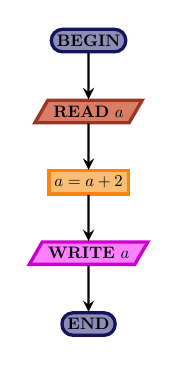
\begin{tikzpicture}[node distance=15mm, scale=0.6, every node/.style={scale=0.6}]
      \node[begin] (start) {\textbf{BEGIN}};
      \node[below of=start,input](in){\textbf{READ} \(a\)};
      \node[below of=in,operation](op){\(a = a+2\)};
      \node[below of=op,output](out){\textbf{WRITE} \(a\)};
      \node[below of=out,begin](end){\textbf{END}};

      \draw[arrow] (start) to (in);
      \draw[arrow] (in) to (op);
      \draw[arrow] (op) to (out);
      \draw[arrow] (out) to (end);
    \end{tikzpicture}\end{center}
    \vfill
  \end{columns}
  \vfill
  \begin{itemize}
    \item \lstinline$std::cin$ è il flusso di input standard
    \vfill
    \item \lstinline$>>$ è l'operatore di \alert{estrazione}
  \end{itemize}
  \vfill
\end{frame}

\begin{frame}[fragile]{Input/Output}
  \vfill
  \begin{lstlisting}
#include <iostream>
int main() {
  std::cerr << "Errore!" << std::endl;
  return 1;
}
  \end{lstlisting}
  \vfill
  \begin{itemize}
    \item \lstinline$std::cerr$ è il flusso su cui comunicare gli errori
    \vfill
    \item Viene gestito diversamente dal sistema operativo
  \end{itemize}
  \vfill
\end{frame}

\begin{frame}[fragile]{Input/Output}
  \vfill
  \begin{lstlisting}
#include <fstream>
int main() {
  std::ofstream fout;
  fout.open("prova.txt");
  fout << "Hello, World!" << std::endl;
  fout.close();
  return 0;
}
  \end{lstlisting}
  \vfill
  \begin{itemize}
    \item \lstinline$<fstream>$ permette di fare input/output su file
    \vfill
    \item \lstinline$std::ofstream$ è un tipo di variabile
    \begin{itemize}
      \item \lstinline$fout$ è il nome della variabile
    \end{itemize}
  \end{itemize}
  \vfill
\end{frame}

\begin{frame}[fragile]{Input/Output}
  \vfill
  \begin{lstlisting}
#include <fstream>
int main() {
  std::ofstream fout;
  fout.open("prova.txt");
  fout << "Hello, World!" << std::endl;
  fout.close();
  return 0;
}
  \end{lstlisting}
  \vfill
  \begin{itemize}
    \item \lstinline$fout.open("prova.txt")$ apre il file \lstinline$prova.txt$
    \vfill
    \item La scrittura avviene come per \lstinline$cout$
    \vfill
    \item \lstinline$fout.close()$ chiude il file
  \end{itemize}
  \vfill
\end{frame}

\begin{frame}[fragile]{Input/Output}
  \vfill
  \begin{lstlisting}
#include <fstream>
int main() {
  std::ofstream fout("prova.txt");
  fout << "Hello, World!" << std::endl;
  fout.close();
  return 0;
}
  \end{lstlisting}
  \vfill
  \begin{itemize}
    \item L'apertura del file può essere fatta nella dichiarazione
  \end{itemize}
  \vfill
\end{frame}

\begin{frame}[fragile]{Input/Output}
  \vfill
  \begin{lstlisting}
#include <iostream>
#include <fstream>
int main() {
  int a;
  std::ifstream fin("dati.txt");
  fin >> a;
  fin.close();
  std::cout << a << std::endl;
  return 0;
}
  \end{lstlisting}
  \vfill
  \begin{itemize}
    \item \lstinline$std::ifstream$ per i file di input
    \vfill
    \item L'operatore \lstinline$>>$ estrae il primo dato nel file
  \end{itemize}
  \vfill
\end{frame}

\begin{frame}[fragile]{Condizionale}
  \vfill
  \begin{columns}[c]
    \column{.45\textwidth}
    \vfill
    \begin{lstlisting}
#include <iostream>
using std::cout;
using std::endl;
int main() {
  int a;
  std::cin >> a;
  if(a == 0) {
    cout << 0 << endl;
  } else {
    cout << 1 << endl;
  }
  return 0;
}
    \end{lstlisting}
    \vfill
    \column{.45\textwidth}
    \vfill
    \begin{center}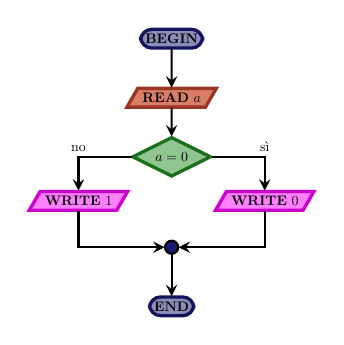
\begin{tikzpicture}[scale=0.5, every node/.style={scale=0.5},node distance=15mm]
      \node[begin] (start) {\textbf{BEGIN}};
      \node[below of=start,input](in){\textbf{READ} \(a\)};
      \node[below of=in,decision](dec){\(a = 0\)};
      \node[below right = 3mm and 8mm of dec,output](pari){\textbf{WRITE} 0};
      \node[below left = 3mm and 8mm of dec,output](dispari){\textbf{WRITE} 1};
      \node[below = 8mm of dec,connection](conn){};
      \node[below of=conn,begin](end){\textbf{END}};

      \draw[arrow] (start) to (in);
      \draw[arrow] (in) to (dec);
      \draw[arrow] (dec) -| node[above] {no} (dispari);
      \draw[arrow] (dec) -| node[above] {sì} (pari);
      \draw[arrow] (dispari) |- (conn);
      \draw[arrow] (pari) |- (conn);
      \draw[arrow] (conn) to (end);
    \end{tikzpicture}\end{center}
    \vfill
  \end{columns}
  \vfill
\end{frame}

\begin{frame}[fragile]{Condizionale}
  \vfill
  \begin{itemize}
    \item \lstinline$if(condizione) { ... } else { ... }$
    \begin{itemize}
      \item il primo blocco viene eseguito se la condizione è vera
      \item il secondo blocco viene eseguito se è falsa
    \end{itemize}
    \vfill
    \item La condizione deve avere un valore di tipo \lstinline$bool$
    \begin{itemize}
      \item spesso risulta da operatori di \alert{confronto}
      \item può contenere espressioni composte
    \end{itemize}
    \vfill
    \item La direttiva \lstinline$else$ può essere omessa
  \end{itemize}
  \vfill
\end{frame}

\begin{frame}[fragile]{Condizionale}
  \vfill
  \begin{itemize}
    \item Operatori di confronto:\\[.5em]
    \hspace{5mm}\begin{tabular}{cl}
      \lstinline$==$ & uguale \\
      \lstinline$!=$ & diverso \\
      \lstinline$>$ & maggiore \\
      \lstinline$>=$ & maggiore o uguale \\
      \lstinline$<$ & minore \\
      \lstinline$<=$ & minore o uguale \\
    \end{tabular}
    \vfill
    \item Operatori logici:\\[.5em]
    \hspace{5mm}\begin{tabular}{cl}
      \lstinline$!$ & not \\
      \lstinline$&&$ & and \\
      \lstinline$||$ & or \\
    \end{tabular}
  \end{itemize}
  \vfill
\end{frame}

\begin{frame}[fragile]{Ciclo while}
  \vfill
  \begin{columns}[c]
    \column{.45\textwidth}
    \vfill
    \begin{lstlisting}
#include <iostream>
using std::cout;
using std::endl;
int main() {
  int a;
  std::cin >> a;
  while(a % 2 == 0){
    a /= 2;
    cout << a << endl;
  }
  return 0;
}
    \end{lstlisting}
    \vfill
    \column{.45\textwidth}
    \vfill
    \begin{center}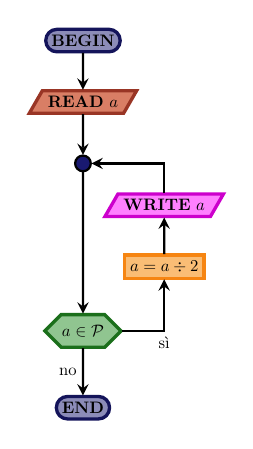
\begin{tikzpicture}[scale=0.6, every node/.style={scale=0.6},node distance=13mm]
      \node[begin] (start) {\textbf{BEGIN}};
      \node[below of=start,input] (read) {\textbf{READ} \(a\)};
      \node[below of=read,connection] (conn) {};
      \node[below right = 3mm and 8mm of conn,output] (write) {\textbf{WRITE} \(a\)};
      \node[below of=write,operation](decr){\(a = a \div 2\)};
      \node[below = 18 mm of conn,loop](loop){\(a \in \mathcal{P}\)};
      \node[below = 6mm of loop,begin](end){\textbf{END}};

      \draw[arrow] (start) to (read);
      \draw[arrow] (read) to (conn);
      \draw[arrow] (conn) to (loop);
      \draw[arrow] (decr) to (write);
      \draw[arrow] (write) |- (conn);
      \draw[arrow] (loop) to node[anchor=east]{no} (end);
      \draw[arrow] (loop) -| node[below]{sì} (decr);
    \end{tikzpicture}\end{center}
    \vfill
  \end{columns}
  \vfill
\end{frame}

\begin{frame}[fragile]{Ciclo while}
  \vfill
  \begin{columns}[c]
    \column{.45\textwidth}
    \vfill
    \begin{lstlisting}
#include <iostream>
using std::cout;
using std::endl;
int main() {
  int a;
  std::cin >> a;
  do {
    a /= 2;
    cout << a << endl;
  } while(a % 2 == 0);
  return 0;
}
    \end{lstlisting}
    \vfill
    \column{.45\textwidth}
    \vfill
    \begin{center}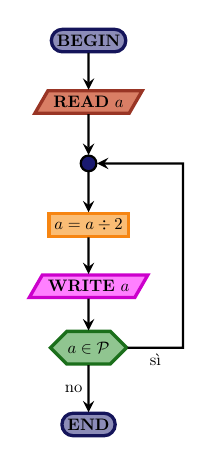
\begin{tikzpicture}[scale=0.6, every node/.style={scale=0.6},node distance=13mm]
      \node[begin] (start) {\textbf{BEGIN}};
      \node[below of=start,input] (read) {\textbf{READ} \(a\)};
      \node[below of=read,connection] (conn) {};
      \node[below of=conn,operation](decr){\(a = a \div 2\)};
      \node[below of=decr,output] (write) {\textbf{WRITE} \(a\)};
      \node[below of=write,loop](loop){\(a \in \mathcal{P}\)};
      \node[below = 6mm of loop,begin](end){\textbf{END}};

      \draw[arrow] (start) to (read);
      \draw[arrow] (read) to (conn);
      \draw[arrow] (conn) to (decr);
      \draw[arrow] (decr) to (write);
      \draw[arrow] (write) to (loop);
      \draw[arrow] (loop) to node[anchor=east]{no} (end);
      \draw[arrow] (loop) to node[anchor=north]{sì} ++(20mm,0) |- (conn);
    \end{tikzpicture}\end{center}
    \vfill
  \end{columns}
  \vfill
\end{frame}

\begin{frame}[fragile]{Ciclo while}
  \vfill
  \begin{itemize}
    \item \lstinline$while(condizione) { ... }$
    \begin{itemize}
      \item ripete il blocco finché la condizione è vera
      \item se la condizione è inizialmente falsa, non entra
    \end{itemize}
    \vfill
    \item \lstinline$do { ... } while(condizione);$
    \begin{itemize}
      \item ripete il blocco finché la condizione è vera
      \item il blocco viene eseguito \alert{almeno} una volta
    \end{itemize}
    \vfill
    \item L'\alert{iterazione} è alla base della programmazione
    \begin{itemize}
      \item sfruttare il computer per fare operazioni ripetitive
    \end{itemize}
  \end{itemize}
  \vfill
\end{frame}

\begin{frame}[fragile]{Ciclo for}
  \vfill
  \begin{columns}[c]
    \column{.6\textwidth}
    \vfill
    \begin{lstlisting}
#include <iostream>
using std::cout;
using std::endl;
int main() {
  int i = 0;
  while(i < 10){
    cout << i << endl;
    i++;
  }
  return 0;
}
    \end{lstlisting}
    \vfill
    \column{.3\textwidth}
    \vfill
    \begin{center}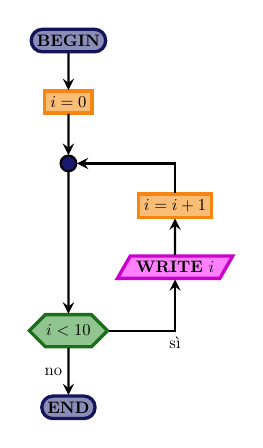
\begin{tikzpicture}[scale=0.6, every node/.style={scale=0.6},node distance=13mm]
      \node[begin] (start) {\textbf{BEGIN}};
      \node[below of=start,operation] (read) {\(i = 0\)};
      \node[below of=read,connection] (conn) {};
      \node[below right = 3mm and 8mm of conn,operation] (write) {\(i = i + 1\)};
      \node[below of=write,output](decr){\textbf{WRITE} \(i\)};
      \node[below = 18 mm of conn,loop](loop){\(i < 10\)};
      \node[below = 6mm of loop,begin](end){\textbf{END}};

      \draw[arrow] (start) to (read);
      \draw[arrow] (read) to (conn);
      \draw[arrow] (conn) to (loop);
      \draw[arrow] (decr) to (write);
      \draw[arrow] (write) |- (conn);
      \draw[arrow] (loop) to node[anchor=east]{no} (end);
      \draw[arrow] (loop) -| node[below]{sì} (decr);
    \end{tikzpicture}\end{center}
    \vfill
  \end{columns}
  \vfill
\end{frame}

\begin{frame}[fragile]{Ciclo for}
  \vfill
  \begin{columns}[c]
    \column{.6\textwidth}
    \vfill
    \begin{lstlisting}
#include <iostream>
using std::cout;
using std::endl;
int main() {
  for(int i = 0; i < 10; i++){
    cout << i << endl;
  }
  return 0;
}
    \end{lstlisting}
    \vfill
    \column{.3\textwidth}
    \vfill
    \begin{center}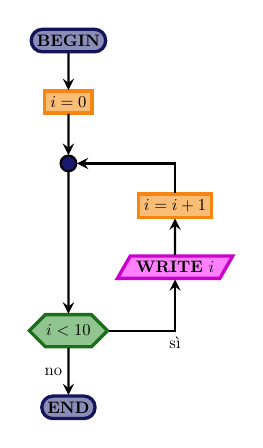
\begin{tikzpicture}[scale=0.6, every node/.style={scale=0.6},node distance=13mm]
      \node[begin] (start) {\textbf{BEGIN}};
      \node[below of=start,operation] (read) {\(i = 0\)};
      \node[below of=read,connection] (conn) {};
      \node[below right = 3mm and 8mm of conn,operation] (write) {\(i = i + 1\)};
      \node[below of=write,output](decr){\textbf{WRITE} \(i\)};
      \node[below = 18 mm of conn,loop](loop){\(i < 10\)};
      \node[below = 6mm of loop,begin](end){\textbf{END}};

      \draw[arrow] (start) to (read);
      \draw[arrow] (read) to (conn);
      \draw[arrow] (conn) to (loop);
      \draw[arrow] (decr) to (write);
      \draw[arrow] (write) |- (conn);
      \draw[arrow] (loop) to node[anchor=east]{no} (end);
      \draw[arrow] (loop) -| node[below]{sì} (decr);
    \end{tikzpicture}\end{center}
    \vfill
  \end{columns}
  \vfill
\end{frame}

\begin{frame}[fragile]{Ciclo while}
  \vfill
  \begin{itemize}
    \item \lstinline$for(iniziale;condizione;incremento) { ... }$
    \begin{itemize}
      \item esegue il comando iniziale
      \item ripete il blocco finché la condizione è vera
      \item al termine di ogni iterazione esegue l'incremento
    \end{itemize}
    \vfill
    \item Utile nel caso sia noto a priori il numero di ripetizioni che un ciclo deve compiere
  \end{itemize}
  \vfill
\end{frame}



\begin{frame}[fragile]{Ciclo for}
  \vfill
  \begin{lstlisting}
#include <iostream>
using std::cout;
using std::endl;
int main() {
  for(int i = 0; i < 10; i++){
    i *= 2;
    cout << i << endl;
  }
  return 0;
}
  \end{lstlisting}
  \vfill
  \begin{itemize}
    \item Cattiva abitudine: cambiare l'indice dentro al ciclo
    \vfill
    \item Cambiare la struttura del ciclo o usare un while
  \end{itemize}
  \vfill
\end{frame}

\end{document}
